\documentclass{article}
\usepackage[utf8]{inputenc}

\documentclass[a4paper]{article}
\usepackage[12pt]{extsizes}
\usepackage{amsmath,amsthm,amssymb}
\usepackage[hidelinks]{hyperref} 
\usepackage[warn]{mathtext}
\usepackage[T1,T2A]{fontenc}
\usepackage[utf8]{inputenc}
\usepackage[english,russian]{babel}
\usepackage{tocloft}
\linespread{1.5}
\usepackage{indentfirst}
\usepackage{setspace}
%\полуторный интервал
\onehalfspacing

\newcommand{\RomanNumeralCaps}[1]
    {\MakeUppercase{\romannumeral #1}}

\usepackage{amssymb}

\usepackage{graphicx, float}
\graphicspath{{pictures/}}
\DeclareGraphicsExtensions{.pdf,.png,.jpg}
\usepackage[left=25mm,right=1cm,
    top=2cm,bottom=20mm,bindingoffset=0cm]{geometry}
\renewcommand{\cftsecleader}{\cftdotfill{\cftdotsep}}

\usepackage{fancyhdr}
\usepackage[nottoc]{tocbibind}

\fancypagestyle{plain}{
\fancyhf{}
\renewcommand{\headrulewidth}{0pt}
\fancyhead[R]{\thepage}
}

\usepackage{blindtext}
\pagestyle{myheadings}
\usepackage{hyperref}

\begin{document}
\begin{titlepage}
  \begin{center}
    \large
    Санкт-Петербургский политехнический университет Петра Великого
    
    Институт прикладной математики и механики
    
    \textbf{Высшая школа прикладной математики и вычислительной физики}
    \vfill
    \textsc{\textbf{\Large{КУРСОВАЯ РАБОТА}}}\\[5mm]
    \\ по дисциплине
    \\ <<Математическая статистика>>\\
\end{center}

\vfill

\begin{tabular}{l p{140} l}
Выполнил студент \\группы 3630102/80401 && Веденичев Дмитрий Александрович \\
\\
Проверил\\Доцент, к.ф.-м.н.& \hspace{0pt} &   Баженов Александр Николаевич \\\\
\end{tabular}

\hfill \break
\hfill \break
\begin{center} Санкт-Петербург \\2021 \end{center}
\thispagestyle{empty}
\end{titlepage}
\newpage
\newpage
\begin{center}
    \setcounter{page}{2}
    \tableofcontents
\end{center}
\newpage
\begin{center}
    \setcounter{page}{3}
    \listoffigures
\end{center}

\newpage

\section{Постановка задачи}
\noindent Есть два набора данных, связанных с красными и белыми вариантами португальского вина "Vinho Verde". Из-за проблем с конфиденциальностью и логистикой доступны только физико-химические (входные данные) и сенсорные (выходные данные) переменные. Данные не сбалансированы, вин среднего качества больше, чем с низкой и высокой оценкой соответственно.

Входные данные представляют собой:
\begin{enumerate}
    \item фиксированную кислотность
    \item летучую кислотность
    \item лимонную кислоту
    \item остаточный сахар
    \item хлориды
    \item свободный диоксид серы
    \item общий диоксид серы
    \item плотность
    \item pH
    \item сульфаты
    \item алкоголь
    \item качество вино
    
\end{enumerate}




\noindent В нашей работе необходимо:
\begin{enumerate}
    \item Считать и обработать полученные наборы данных.
    \item Обучить наивный байесовский классификатор с помощью тренировочных данных.
    \item Провести тестирование обученного классификатора и исследовать результаты.
\end{enumerate}

\section{Теория}
Часто бывает необходимо определить принадлежность объекта какому-то классу. Для данной задачи используются инструменты, называемые классификаторами. Одним из них является наивный Байесовский классификатор, который основан на применении теоремы Баейса со строгими (наивными) предположениями о независимости определяющих объект характеристик. В зависимости от природы вероятностной модели, Байесовский наивный классификатор способен показывать результаты лучше чем обучаемые нейросети. Это, в совокупности с возможностью обучаться по малым объемам данных, делает из него серьезный инструмент для решения жизненных задач.

\subsection{Модель наивного Байесовского классификатора}
Вероятностная модель для классификатора — это условная модель $p(Class|X_1,X_2,..,X_n)$ над зависимой переменной $Class$ с малым количеством значений (классов) от нескольких переменных $X_1,X_2,..,X_n$.  Используя теорему Байеса запишем: $$p(Class|X_1,X_2,..,X_n)= \frac{p(Class)p(X_1,X_2,..,X_n|Class)}{p(X_1,X_2,..,X_n)}$$

На практике интересен лишь числитель, так как знаменатель не зависит от $Class$, и значения свойств $X_i$ даны, так что знаменатель - константа.
Числитель эквивалентен совместной вероятности модели $p(Class,X_1,...,X_n)$, для которой можно выполнить следующие преобразования
$$p(Class,X_1,...,X_n)= p(Class)p(X_1,..,X_n|Class)=p(Class)p(X_1|Class)p(X_2,...,X_n|Class,X_1)=$$ 
$$=p(Class)p(X_1|Class)...p(X_n|Class,X_1,...,X_{n-1})$$

Используем 'наивное' предположение о независимости переменных, которое позволяет нам сделать преобразование $p(X_i|Class,X_j)=p(X_i|Class), i \neq j$.
Тогда полученное выше можно преобразовать в виде 
$$p(Class,X_1,...,X_n)=p(Class)p(X_1|Class)...p(X_n|Class,X_1,...,X_{n-1})=$$ $$=p(Class)p(X_1|Class)...p(X_n|Class)=p(Class)\prod_{i=1}^n p(X_i|C)$$

Таким образом, из предположения о независимости, условное распределение $Class$ можно выразить в виде
$$p(Class|X_1,X_2,..,X_n)=\frac{1}{Z}p(Class)\prod_{i=1}^n p(X_i|C)$$

Где $Z = p(X_1,..,X_n)$ - это коэффициент масштабирования, зависящий только от $X_1,..,X_n$, таким образом это  константа, если значения известны.
\subsection{Оценка параметров и построенние классификатора по модели}

Параметры модели могут быть аппроксимированы относительными частотами из набора данных обучения. Это оценки максимального правдоподобия вероятностей. Непрерывные свойства, обычно оцениваются через нормальное распределение. Для математического ожидания и дисперсии вычисляются среднее арифметическое и среднеквадратическое отклонение.

Наивный Байесовский классификатор объединяет Баейсовскую модель(2.1) с правилом решения. Одно общее правило должно выбирать наиболее вероятную гипотезу, оно также известно как апостериорное правило принятия решения (MAP). Соответствующий наивный Баейсовский классификатор — это функция  определённая следующим образом: $$classify(x_1,...,x_n)=\underset{Сlass}{\rm argmax}\ p(Class=class)\prod_{i=1}^n p(X_i=x_i|Class=class) $$

\section{Программная реализация}
\noindent Код программы был написан на языке Python в среде разработки PyCharm. В ходе работы использовались дополнительные библиотеки:
 \begin{enumerate}
        \item seaborn
        \item matplotlib 
        \item numpy 
        \item pandas
        \item sklearn
    \end{enumerate}
В приложении находится ссылка на GitHub репозиторий с исходныи кодом.

\section{Ход работы}
На вход подаются два .csv файла с данными о красном и белом винах. Все последующие этапы описывают взаимодействие с одним из двух файлов. Таким образом рассматривается один тип вина за итерацию работы.
\begin{enumerate}
    \item Обработка данных. Данные из файла собираются в pandas.dataframe. Выполняется проверка на наличие отсутствующих значений. Составление таблицы корреляции переменных в датасете. Для упрощения задачи классификации, количество классов с 11 (от 0 до 10) уменьшается до 2. Теперь от 0 до 6.5 будет 'плохое' вино(ему соотвествует 0), от 6.5 до 10 'хорошее' вино(ему соответствует 1). Данное упрощение связано как с недостатком данных для крайних значений, так называемой несбалансированностью, так и с упрощением работы для классификатора.
    \item Создание тренировочных и тестовых датасетов. Разбиваем исходные данные на тренировочные и тестовые, используя встроенные функции sklearn. Перед разделением на тестовые и тренировочные данные -  датасет перемешивается. Тестовые данные будут составлять 20\% от входных данных. Каждый из тренировочных и тестовых датасетов представляет из себя два элемента: матрица, где на строках представлены значения $x_i$, и вектор, где элементами являются зависимые переменные $c_i$.
    \item Обучить классификатор на тренировочных данных. Тренировочные данные, полученные на предыдущем этапе, используются для обучения классификатора.
    \item Проверить классификатор на тестовых данных. Получить предсказания от классифиактора на тестовых данных. Сравнить предсказания с имеющимися ответами. Собрать результаты сравнения.
    \item Отобразить метрики. Из собранных данных отобразить результат обучения классификатора.
\end{enumerate}

\section{Результаты}
\subsection{Корреляция переменных в исходных датасетах}
\begin{figure}[H]
		\centering
		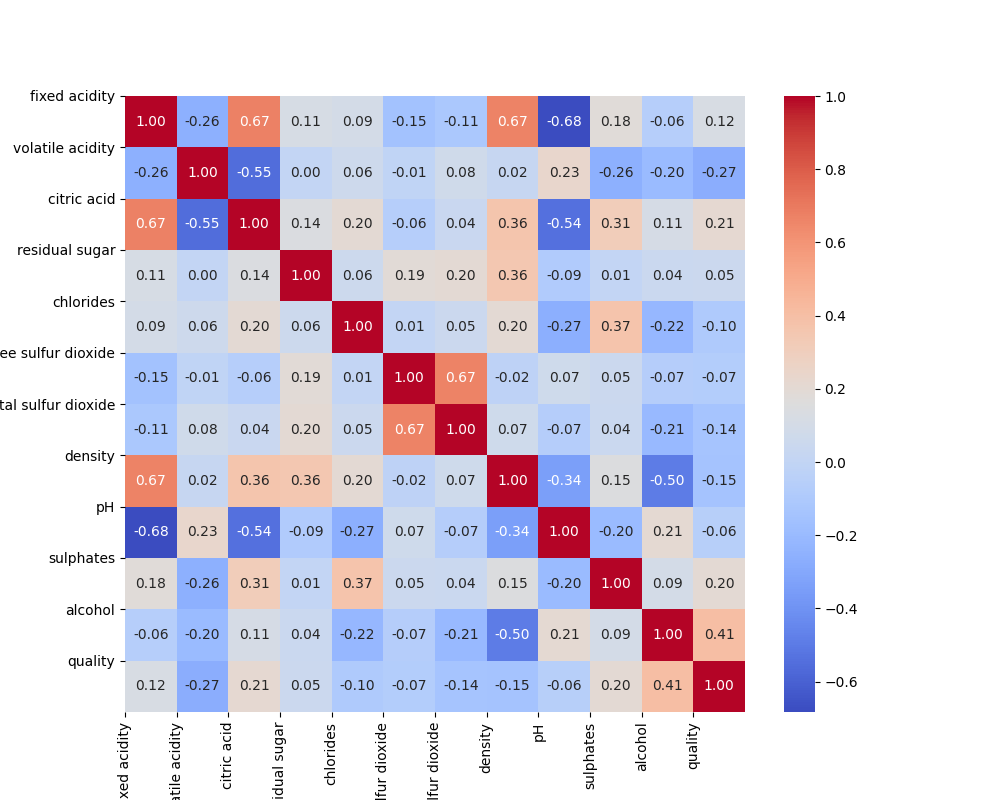
\includegraphics[width = 15cm, height = 9cm]{red_cor.png}
		\caption{Корреляция переменных в красном вине}
	\end{figure}
	
\begin{figure}[H]
		\centering
		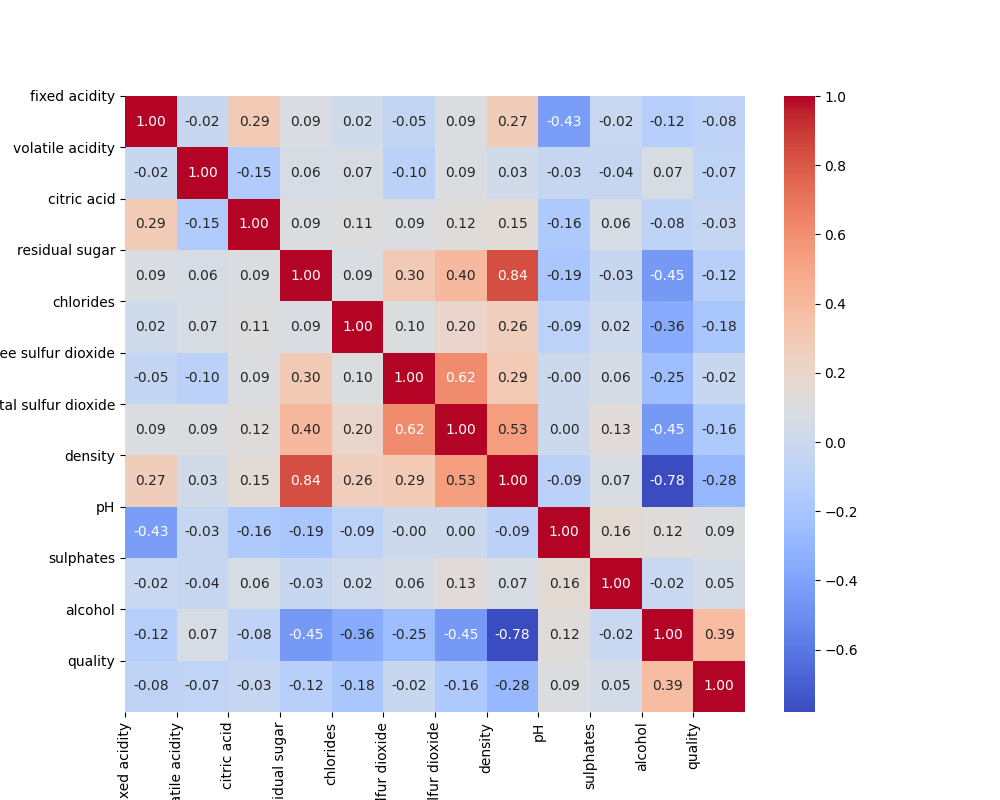
\includegraphics[width = 15cm, height = 9cm]{white_cor.png}
		\caption{Корреляция переменных в белом вине}
	\end{figure}
	
\subsection{Результаты классификации наивным Баейсовским классификатором}
	
\begin{figure}[H]
		\centering
		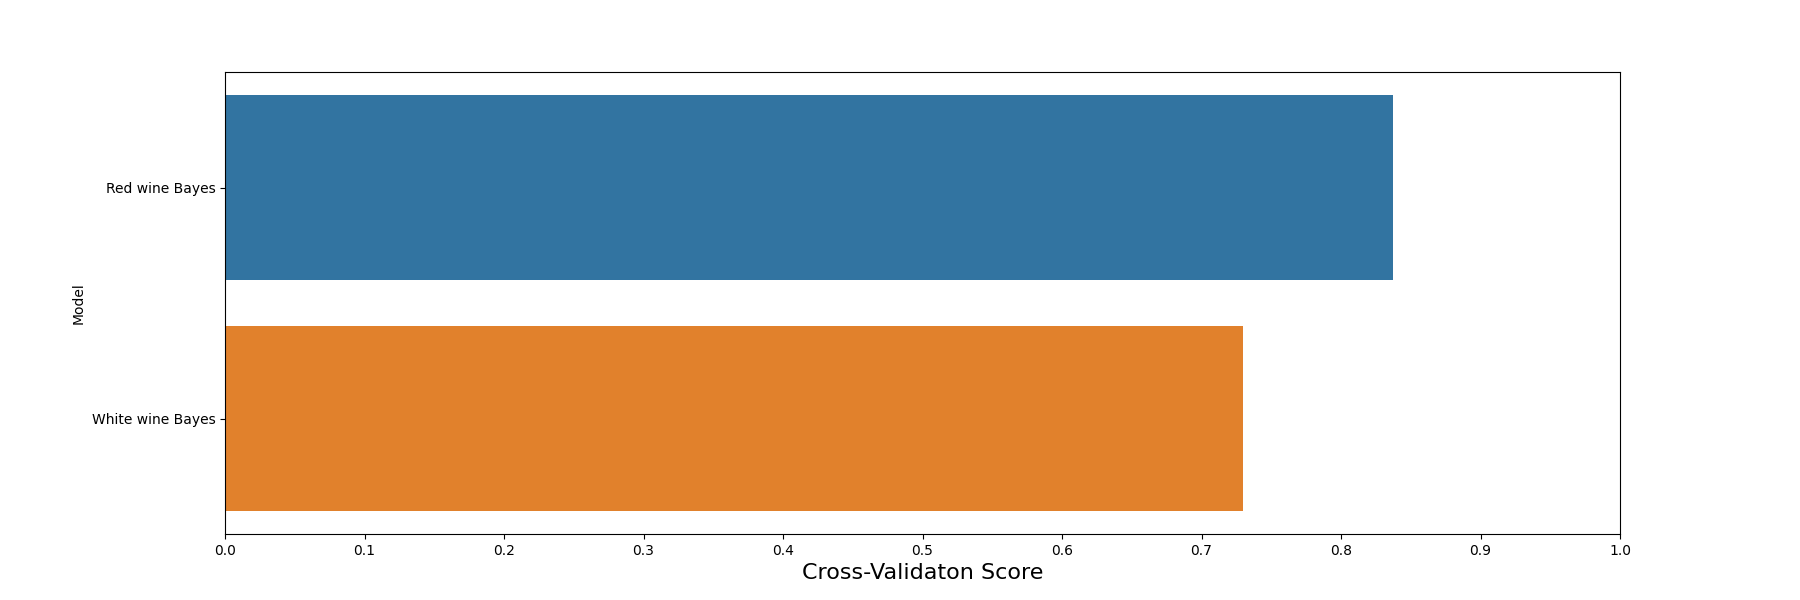
\includegraphics[width=0.95\paperwidth]{cros_val_test.png}
		\caption{Результаты перекрестной проверки классификаторов белого и красного вина}
	\end{figure}
	
	
\begin{table}[H]
    \centering
    \begin{tabular}{c|p{1.5 cm}|p{1.5 cm}|p{1.5 cm}|p{1.5 cm}|p{1.5 cm}|p{1.5 cm}|p{1.5 cm}}
         Model & True Positive & False Positive  &True Negative&  False Negative&  Accuracy (training) & Accuracy (test) & Cross-Validation\\\hline
 White wine Bayes &539     &      214  & 159  & 68     &0.732   &    0.712   &  0.730   \\   
 Red wine Bayes   &234 &  39 &    37    &    10   &  0.839  &          0.847   &     0.837 
    \end{tabular}
    \caption{Матрица ошибок}
    \end{table}

\section{Анализ}
При изучении графика (3) и таблицы (1) получаем следующее: \\
Наивный Баейсовский классификатор показывает хороший результат в классификации красных вин, несмотря на малый размер датасета. Белые вина имеют больший датасет, однако классификатор показывает себя хуже, чем с красных вином.
	
\section{Приложение}
\noindent Код программы GitHub URL:\\
\newline https://github.com/PopeyeTheSailorsCat/Bayes\_estimator-mat\_stat\_course-/tree/main/src

\begin{thebibliography}{9}

\bibitem{book1} Hand, DJ, & Yu, K. (2001). «Idiot’s Bayes — not so stupid after all?» International Statistical Review. Vol 69 part 3, pages 385—399.
\bibitem{book2} J.P. Sacha. "New synthesis of Bayesian network classifiers and interpretation of cardiac SPECT images", Ph.D. Dissertation, University of Toledo, 1999., page 48
\bibitem{book3} Электронный ресурс: https://scikit-learn.org/stable/modules/naive\_bayes.html
\bibitem{book4} Электронный ресурс: https://nlp.stanford.edu/IR-book/html/htmledition/naive-bayes-text-classification-1.html

\end{thebibliography}

\end{document}